% LATeX2e document

\documentclass[12pt]{article}
\pagestyle{empty}

\usepackage{tikz-cd}
\usepackage{amsmath,amssymb,amsfonts,bm}
\usepackage{stmaryrd}
\usepackage{bbold}
\usepackage{times}
\usepackage[all]{xy}
\usepackage{mathrsfs}
\usepackage{graphicx}
\usepackage{url}
\usepackage{pgfplots}
\usepackage{xcolor}
\usepackage{amsthm}
\usepackage[space]{grffile}
\usepackage{float}

\floatstyle{boxed} 
\restylefloat{figure}
\graphicspath{ {C:/Users/Geoffrey/} }
\pgfplotsset{compat=1.12}
\textwidth 1.2\textwidth
\textheight 1.2\textheight
\topmargin 0in
\oddsidemargin 0in
\setlength{\topmargin}{0in}
\setlength{\headsep}{0in}
\setlength{\headheight}{0in}

%%%%%%%%%%%%%%%%%   definitions    %%%%%%%%%%%%%%%%%%%%%%%%%%%%%%%%%%%%

\DeclareMathOperator{\Log}{log}
\DeclareMathOperator{\WN}{WordNorm}
\DeclareMathOperator{\WNt}{WordNormCtrl}
\DeclareMathOperator{\WNp}{WordNormComp}
\DeclareMathOperator{\TS}{TextScore}
\DeclareMathOperator{\atanh}{arctanh}
\DeclareMathOperator*{\mean}{Mean}

\newcommand{\onto}{\twoheadrightarrow}
\newcommand{\mono}{\rightarrowtail}
\newcommand{\into}{\hookrightarrow}
\newcommand{\tto}{\longrightarrow}
\newcommand{\iso}{\overset{\sim}{\tto}}
\newcommand{\impl}{\Rightarrow}
\newcommand{\conj}[1]{{}^#1}
\newcommand{\bigslant}[2]{\raisebox{.2em}{$#1$}\left/\raisebox{-.2em}{$#2$}\right.}

\newcommand{\bs}{\mspace{0mu}}
\newcommand{\ednote}[1]{\textcolor{red}{#1}}

\newcommand*{\codefont}{\fontfamily{cmvtt}\selectfont}

%\renewcommand{\labelenumi}{(\alph{enumi})}
\renewcommand{\labelenumi}{\textbf{(\alph{enumi})}}

\definecolor{o5}{RGB}{247,163,46}
\definecolor{o4}{RGB}{249,181,88}
\definecolor{o3}{RGB}{250,200,130}
\definecolor{o2}{RGB}{252,218,171}
\definecolor{o1}{RGB}{253,237,213}
\definecolor{w}{RGB}{255,255,255}
\definecolor{b1}{RGB}{209,213,252}
\definecolor{b2}{RGB}{163,171,250}
\definecolor{b3}{RGB}{116,130,247}
\definecolor{b4}{RGB}{70,88,245}
\definecolor{b5}{RGB}{242,46,242}

\newtheorem{definition}{Definition}

\title{What is the Difference Between Data Science and Machine Learning?}
\date{\today}
\author{Geoffrey E. Schneider}

\begin{document}

\maketitle
\section{Introduction} Data science is the practice of extracting useful information from data. Machine learning is a set of programming techniques in which the programmer sets up a model with variable parameters and a method by which these parameters will be "learned" from data. There. Question answered. In practice, however, when searching for a job, it isn't so clear. Because of the large overlap between the two, a job listed as a data science job may really be more of a machine learning job, and vice versa. And perhaps you want to pick up a few new, relevant skills, but you are interested in one of the two fields, and not the other. Can we disentangle which skills are more relevant to your chosen field from the job descriptions posted for applicants?

The goal of this project is to use textual analysis to solve this issue. We start with a standard set of methods, using Support Vector Machines (SVMs) with and without Word2Vec. This, however, has the disadvantage that it only provides a method for distinguishing, but no more detailed analysis. So, we move on to an original method we call WordNorm, which adds a numerical value that quantifies the extent to which a document lies in data science v.s. machine learning, and also gives a word-by-word analysis, in addition to distinguishing. The SVMs were created using the Python package sklearn, and Word2Vec was implemented in TensorFlow. Code for WordNorm was written in the new and exciting programming language Julia \cite{Julia}. This document was produced using \LaTeX\, PyPlot (for most figures) and Julia (some figures are from \LaTeX\ code produced by Julia code).

\section{Data} The data for this project is 150 posted job descriptions\cite{LinkedIn}. They are divided into three datasets, the machine learning descriptions (50), the data science descriptions (50), and the control descriptions (50). These were gathered by doing searches for the relevant words ("machine learning job"/"data science job"/"job"), and then divided into sequences of words using regular expressions. In Julia this is implemented as:

\begin{verbatim} 
function texttowords(text)
  matchall(
    r"(\w+)",
    lowercase(replace(text, r"([\r\n,\.\(\)!;:\?/]|\ufeff)", s" "))
    )
end
\end{verbatim}
(and similarly in Python). The sequences of words were then divided into "bags of words" (i.e. word counts), one for each of the datasets.

\begin{verbatim}
function wordcount(wordvec)
  worddict = Dict{String,Int64}()
  for w in wordvec
    worddict[w]=get(worddict,w,0) + 1
  end
  worddict
end
\end{verbatim}

\section{Methods}
\subsection{SVMs and Word2Vec} Linear Support Vector Machines give a simple method for distinguishing between two classes given as data points in a (possibly high-dimensional) space by finding a hyperplane that divides them as well as is possible. More general SVMs could easily be used, but were found to provide no advantage in this setting.

In order to encode a document as a point in space, we can do several things. The simplest approach is to use the one-hot encoding for the individual words (so each is viewed as a standard basis vector a space with dimension equal to the number of words), and then average the vectors representing these words in a document to get a vector representing each document. In our corpus of job descriptions there are 5944 distinct words, meaning that the space in which our data is represented is 5944-dimensional. Having this many features (each dimension represents a feature of the document, i.e., how many of a particular word is in that document) with only 100 examples (150 if you include control documents) is not good, and may affect generalizability of this method. To fix this, we can compress our encoding using the standard Word2Vec CBOW method (which has the added advantage of using the data of the word order to define the encoding, data which would otherwise be thrown away).

Briefly, Word2Vec is a method similar to that of autoencoders, in which we obtain an encoding for words from the first half of a neural net which first encodes the words, and then tries to do some task with the encoded word. Unlike autoencoders, with Word2Vec we are not reconstructing the word (as the word itself has no structure, and so the encoding obtained by this wouldn't reflect anything about the word), but instead we try to fill in the blank from a sequence of words extracted in order from text. In this case, we train the Word2Vec network to guess the middle word in a sequence of five words from the other four. We use a simple 2-layer net in which the first layer encodes the four outer words, and then next guesses the middle word from the encoded outer words.

\subsection{WordNorm} To compare two of the datasets, we will use two variations on what we will call "WordNorm" (for non-technical folks, you can skip from here to the tldr at the end if this section, if you want). For datasets $\alpha$ and $\beta$ (e.g. $\alpha = \text{data science}$ and $\beta = \text{control}$) and word $w$, the ideal version of WordNorm
\begin{equation} \label{eqn:WordNorm}
 \WN_{\alpha\beta}(w) = \frac{\alpha(w)-\beta(w)}{\alpha(w)+\beta(w)}
\end{equation}
where $\alpha(w)$ (resp. $\beta(w)$) indicates the word count for $w$ in $\alpha$. We will write $\WN(w)$ when the choice of $\alpha$ and $\beta$ are clear or irrelevant. Note that 
\[
 \WN(w) = \begin{cases} 1 & w \in \alpha \smallsetminus \beta \\ -1 & w \in \beta \smallsetminus \alpha \end{cases}
\]
and that $1$ and $-1$ are the maximum and minimum values of $\WN$. So, if $w$ is near $1$, it is much more closely associated to $\alpha$, and if $w$ is near $-1$, it is much more closely associated to $\beta$. In an ideal setting, with a very large amount of data (so that each word count has at least one of each word), this would work well, however in a practical setting there is an issue. For example, suppose we're interested in comparing the word "dog" to the word "cat", and $\alpha(\text{"dog"}) = 5$, $\alpha(\text{"cat"}) = 1$, but $\beta(\text{"dog"})=\beta(\text{"cat"})=0$. $\WN$ does not distinguish between "dog" and "cat"! $\WN(\text{"dog"})=\WN(\text{"cat"}) = 1$, despite the fact that it is clear that $\alpha$ is probably more strongly associated with "dog" than it is with "cat". To deal with this problem, we will use the two modifications that follow.

When comparing a sample dataset $\alpha$ (e.g. the counts of words in machine learning job descriptions) to the control dataset (which we write as $c$) we use
\begin{equation} \label{eqn:WordNormCtrl}
 \WNt_\alpha(w) = \frac{\alpha(w) - (c(w)+1)}{\alpha(w) + (c(w) + 1)}
\end{equation}
where we've written the parentheses to emphasize the interpretation that $\WNt$ is just $\WN$ where we've added one of each word to the control dataset. Now using $\beta$ in the example above as a control, we get $\WNt(\text{"dog"})=\frac{2}{3}$ and $\WNt(\text{"cat"})=0$. For our setting $\WNt$ has the nice feature that common words ("is", "the", etc.) and general job words ("applicant", "responsibilities") get a score close to $0$, and so when we are looking at the top scores, these are automatically ignored. It loses the (anti)symmetry of $\WN$, but this is acceptable, because the sample and control are playing different roles here.

When comparing two sample datasets, we can use
\begin{equation} \label{eqn:WordNormComp}
 \WNp_{\alpha\beta}(w) = \frac{\alpha(w) - \beta(w)}{\alpha(w) + \beta(w) +1}.
\end{equation}
This is equivalent to adding half a count of each word to both datasets. In a sense, we are saying that we expect that if $\alpha(w)=0$, the "real value" of $\alpha(w)$ is between 0 and 1, but we need a larger sample to determine the value, so we guess that it is $0.5$, but then to be fair to the other words where $\alpha(w)>0$, we also add $0.5$ to their counts. Here the (anti)symmetry is restored, as it should be since both datasets play interchangeable roles.

Finally, to score a full document, we could try to naively take the average score of its words, but this would be a bad approach because there is a skewed level of importance for $\WN$ scores close to $\pm 1$. To understand this issue, consider what happens when we average a word with a score of $0.99$ with a word with a score of $0.00$ (using $\WNp$). The score of $0.99$ might represent 298 examples in the first dataset and 1 in the second, whereas a score of $0.00$ might represent 1 example in the first and 1 in the second. The average is $\approx 0.50$, which is the same as the average of two words with scores of $0.50$ each representing 4 examples in the first dataset and 1 in the second. Clearly, this is a problem for the naive average. To fix this issue, we can transform the range of $\WNp$ (from $(-1,1)$ to $(-\infty, \infty)$) by taking the inverse hyperbolic tangent, averaging these transformed scores, and then inverting the transformation, taking the hyperbolic tangent of the average. Written in mathematical notation this is
\begin{equation} \label{eqn:TextScore}
 \widehat{\TS}(\text{text}) = \tanh(\mean_{w \in \text{text}}(\tilde{w}))
\end{equation}
where $\tilde{w} = \atanh(\WNp(w))$. TextScore should be interpreted relative to the score on a control dataset, so we introduce a modified version of the above score
\begin{equation} \label{eqn:modTS}
 \TS(\text{text}) = \tanh(\mean_{w \in \text{text}}(\tilde{w}-\atanh(\widehat{\TS}(\text{control}))))
\end{equation}
\\
 
\noindent [\textit{tldr: There are a few variations of $\WN$, but in all cases, it assigns a value between 1 and -1 to each word. 1 means the word is much more closely associated to the dataset, and -1 means the word is much more closely associated to the second. When one of these is the control, it will always be the second. $\TS$ is a kind of average $\WN$ over an entire document.}]

\section{Results and Discussion}
\subsection{SVMs and Word2Vec} First, using a Linear SVM on the unencoded representation of words, we obviously successfully divide the training set into two regions giving a training accuracy of 100\%, but on the validation set, we only obtain an accuracy of 60\% (6 put of 10 documents correctly classified). This justifies the addition of Word2Vec embeddings.

Using a Word2Vec embedding into two dimensions (see Figure \ref{fig:trainW2V2} for the training data) allows us to visualize the resulting embeddings, as shown in Figure \ref{fig:W2VEmb}. As expected, we see that this does not immediately introduce a classification of words into data science vs machine learning associated words, however we do see some semantic information being reproduced, for example the words representing frameworks for implementing (parts of) machine learning ('apache', 'torch', 'caffe', 'tensorflow') all cluster in the same region.

\begin{figure}[h]
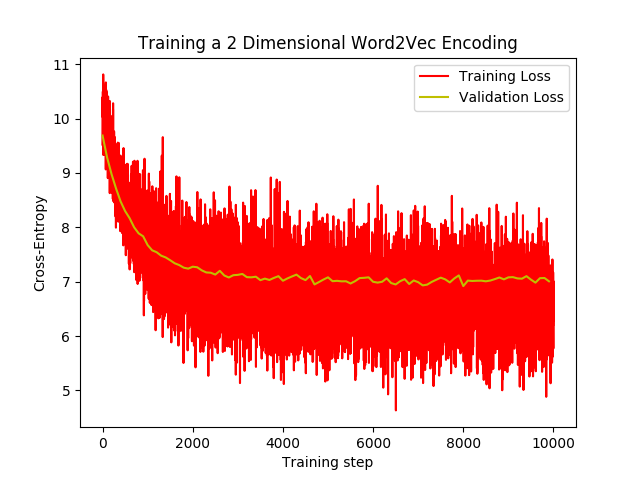
\includegraphics[scale=1]{C:/Users/Geoffrey/Documents/Job_descriptions/TrainingW2V2.png}
\caption{\label{fig:trainW2V2} Training curves for 2-dimensional Word2Vec. Note that the validation curve continues to fall (though slowly at the end) throughout the training, however, training and validation loss begin to diverge near the end of training.}
\end{figure}

\begin{figure}[h]
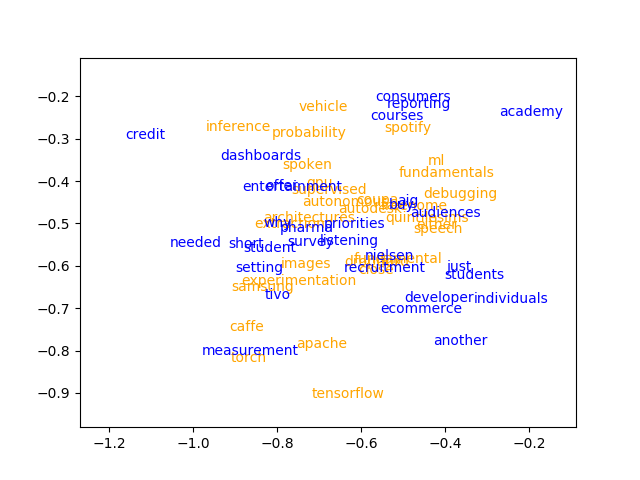
\includegraphics[scale=1]{C:/Users/Geoffrey/Documents/Job_descriptions/W2VplotTop30.png}
\caption{\label{fig:W2VEmb} Embeddings of selected words in 2-dimensional space using Word2Vec. Words chosen were the highest WordNorm scoring words for data science and machine learning, colored according to the category in which they scored highly.}
\end{figure}

Though a 2-dimensional representation is nice for visualization, using it with an SVM does not allow us to separate data science job descriptions from machine learning ones (see Figure \ref{fig:SVM2d}). On the validation set, this SVM correctly identified 50\% of the job descriptions.

\begin{figure}[h]
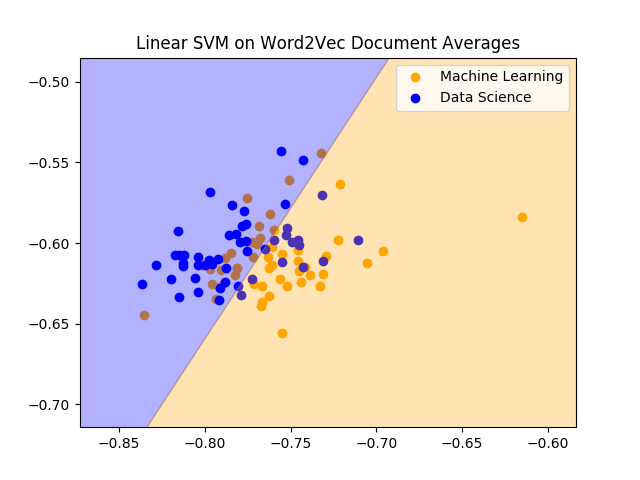
\includegraphics[scale=1]{C:/Users/Geoffrey/Documents/Job_descriptions/2dsvm.png}
\caption{\label{fig:SVM2d} Using a Linear SVM on the scores for data science vs machine learning job descriptions from a 2-dimensional implementation of Word2Vec.}
\end{figure}

Using higher dimensional embeddings will allow us to get a better performance. Using a 10-dimensional encoding we get an 80\% accuracy on the validation set and using a 100-dimensional encoding gives a 90\% accuracy on the validation set. We conclude that the 100-dimensional encoding is the best choice for this task. The test set also gives a 90\% accuracy for the 100-dimensional embedding. Figure \ref{fig:100dsvm} shows a projection of the 100-dimensional embedding down to 2 dimensions.

\begin{figure}[h]
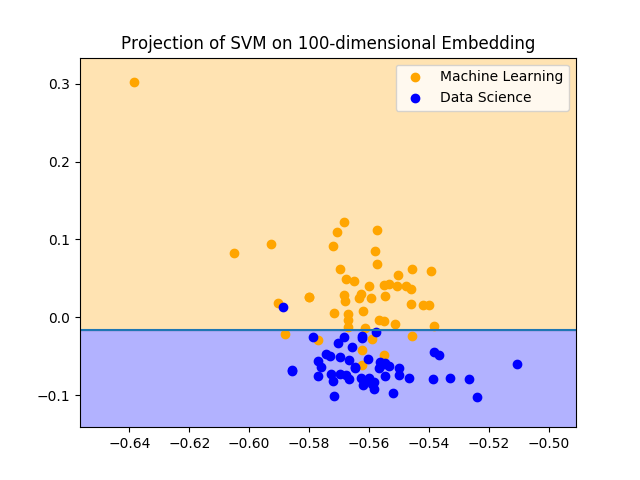
\includegraphics[scale=1]{C:/Users/Geoffrey/Documents/Job_descriptions/100dsvm.png}
\caption{\label{fig:100dsvm} The 100 dimensional embedding projected down to 2 dimensions, such that the dividing hyperplane is a line. This visualization includes the training, validation and test sets.}
\end{figure}

\subsection{WordNorm} In Figure \ref{fig:WNt} we show the results of applying $\WNt$ to data science (vs. control) and to machine learning (vs. control). We see that the two give broadly similar scores validating the assertion that there is much overlap between the two. Languages such as R, Python and Spark, as well as the distributed system framework Hadoop appear in the top 10 for both.

For "visualization" we see a higher data science score, confirming the stronger importance of communicating findings to allow companies to make informed business decisions, whereas the higher machine learning score for "ai" indicates the importance of building automated systems as a product in themselves. The word "academy" appears at first to be strongly associated with data science and strongly dissassociated with machine learning, however, it is an aberration which should be ignored, as it is on this list only because it appeared a very large number of times in one particular data science job description, and not at all in the control and machine learning data.

\begin{figure}[h]
\begin{center}
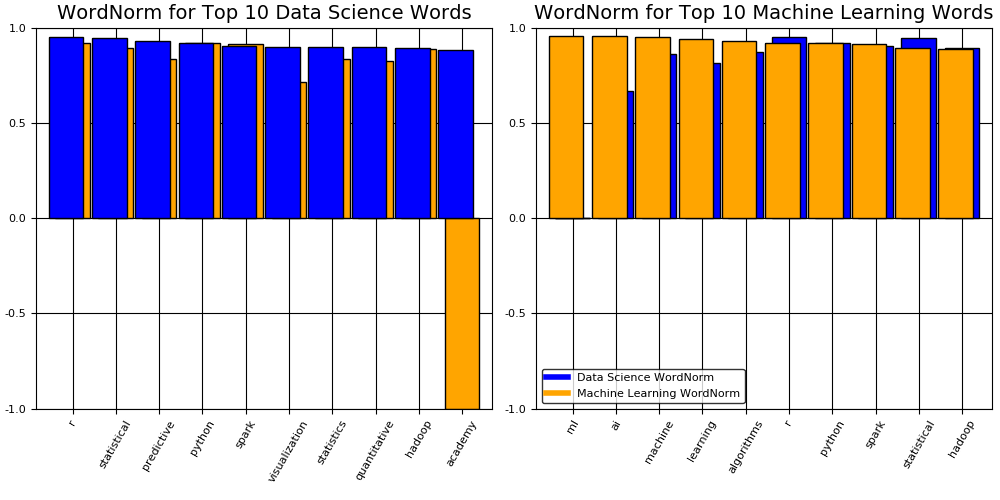
\includegraphics[scale=0.6]{C:/Users/Geoffrey/Documents/Job_descriptions/WordNormTop10.png}
\end{center}
\caption{\label{fig:WNt} The words with the highest $\WNt$ scores for both data science and machine learning.}
\end{figure}

Comparing the data science and machine learning data to the control tells us a lot about what is important to each of them, but due to their large overlap, it does not allow us to \textit{distinguish} them. To do this, we compare them directly using $\WNp$. Figure \ref{fig:WNp} shows the result of applying $\WNp_{ml,ds}$ to directly compare machine learning to data science.

Machine learning frameworks TensorFlow and Caffe are both represented with a stronger association with machine learning whereas words like "consumers" and "audiences" are associated with data science. We also see the names of companies that are associated with machine learning or data science. These company names may be due to the inclusion of jobs advertised by those companies in the dataset, though this is not entirely clear in the case of software companies, where the inclusion may be due to requirements that applicants have knowledge of their software. 

\begin{figure}[h]
\begin{center}
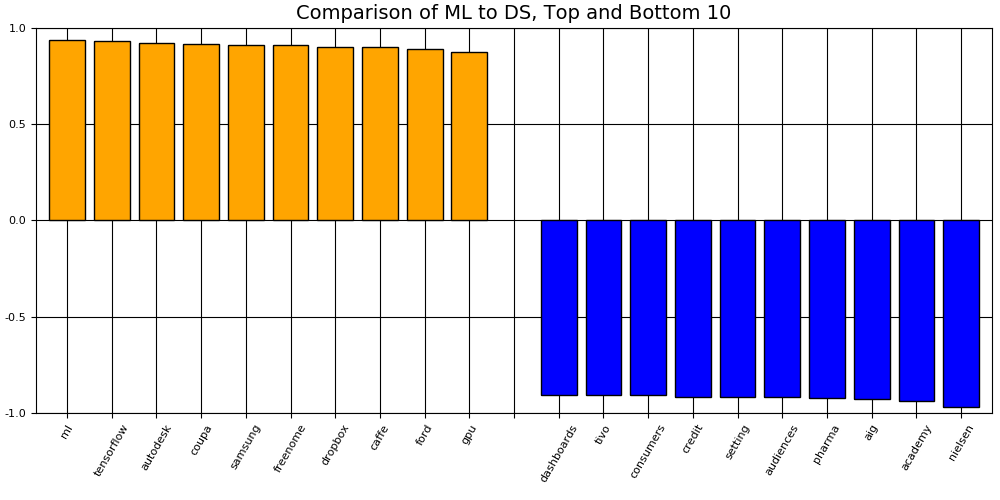
\includegraphics[scale=0.6]{C:/Users/Geoffrey/Documents/Job_descriptions/MLvsDS.png}
\end{center}
\caption{\label{fig:WNp} The result of comparing machine learning to data science with $\WNp$. Positive scores indicate stronger association with machine learning, and negative scores indicate stronger association with data science.}
\end{figure}

Using the $\TS$, we can score any text in terms of whether it is more closely associated with data science or machine learning\footnote{On the concatenation of the documents that made up the control dataset, the $\widehat{\TS}$ is $-0.143$, and so all $\TS$ scores following are normalized by this value.}. Note that because this is a kind of average, we should expect scores to be closer to 0 than on individual words. On an additional data science job description, the $\TS$ was $-0.084$. On an additional machine learning job description the $\TS$ was $0.103$. The first two pairs of texts in Figure \ref{fig:TextColored} show the first 50 words of these document, words colored according to their $\WN$\footnote{Normalized by the $\widehat{\TS}$ of the control.}.

We can even try this on documents that are not directly descriptions of a particular job. For example, the Insight Data Science Fellows Program has a white paper with a section titled "What is a Data Scientist?"\cite{InsightWP}. The third pair of texts Figure \ref{fig:TextColored} shows the first 50 words of this document, each colored according to their $\WNp$ score. The overall $\TS$ for this document is slightly less than 0, at $-0.005$.

\begin{figure}[h]
our clients seeks an experianced leader who will sit at the intersection of analytics data management it software infrastructure in the center for data science and analytics is an innovative corporate analytics group within the business they are a rapidly growing entrepreneurial department which aims to design create and offer

{\color{b1}our} {\color{b2}clients} {\color{o1}seeks} {\color{w}an} {\color{o1}experianced} {\color{b2}leader} {\color{b1}who} {\color{w}will} {\color{o1}sit} {\color{w}at} {\color{b1}the} {\color{o1}intersection} {\color{w}of} {\color{b3}analytics} {\color{b1}data} {\color{b2}management} {\color{b1}it} {\color{o2}software} {\color{o3}infrastructure} {\color{w}in} {\color{b1}the} {\color{b2}center} {\color{w}for} {\color{b1}data} {\color{b2}science} {\color{w}and} {\color{b3}analytics} {\color{w}is} {\color{w}an} {\color{b1}innovative} {\color{b2}corporate} {\color{b3}analytics} {\color{o1}group} {\color{b2}within} {\color{b1}the} {\color{b2}business} {\color{b2}they} {\color{w}are} {\color{w}a} {\color{w}rapidly} {\color{b1}growing} {\color{o1}entrepreneurial} {\color{b1}department} {\color{b1}which} {\color{o1}aims} {\color{w}to} {\color{b1}design} {\color{w}create} {\color{w}and} {\color{o1}offer}\\

machine learning researcher this is a new role designed for a new and unexplored environment designing machine learning and deep learning algorithms you will have petabytes of data state of the art hardware such as massive distributed clusters and gpus and professional support to develop ways to design complex and

{\color{o3}machine} {\color{o3}learning} {\color{o1}researcher} {\color{b1}this} {\color{w}is} {\color{w}a} {\color{b1}new} {\color{b2}role} {\color{b1}designed} {\color{w}for} {\color{w}a} {\color{b1}new} {\color{w}and} {\color{o1}unexplored} {\color{w}environment} {\color{o1}designing} {\color{o3}machine} {\color{o3}learning} {\color{w}and} {\color{o2}deep} {\color{o3}learning} {\color{o2}algorithms} {\color{w}you} {\color{w}will} {\color{o1}have} {\color{o1}petabytes} {\color{w}of} {\color{b1}data} {\color{b1}state} {\color{w}of} {\color{b1}the} {\color{o1}art} {\color{o1}hardware} {\color{o2}such} {\color{w}as} {\color{o1}massive} {\color{o2}distributed} {\color{o4}clusters} {\color{w}and} {\color{o1}gpus} {\color{w}and} {\color{w}professional} {\color{w}support} {\color{w}to} {\color{o1}develop} {\color{b1}ways} {\color{w}to} {\color{b1}design} {\color{b1}complex} {\color{w}and}\\

the amount of data produced across the globe has been increasing
exponentially and will continue to grow at an accelerating rate for the foreseeable future at companies across all industries servers are overflowing with usage logs message streams transaction records sensor data business operations records and mobile device data effectively

{\color{b1}the} {\color{o2}amount} {\color{w}of} {\color{b1}data} {\color{o1}produced} {\color{b1}across} {\color{b1}the} {\color{b1}globe} {\color{b1}has} {\color{b2}been} {\color{o1}increasing} {\color{o1}exponentially} {\color{w}and} {\color{w}will} {\color{o1}continue} {\color{w}to} {\color{b1}grow} {\color{w}at} {\color{w}an} {\color{o1}accelerating} {\color{o4}rate} {\color{w}for} {\color{b1}the} {\color{o1}foreseeable} {\color{b1}future} {\color{w}at} {\color{b2}companies} {\color{b1}across} {\color{b1}all} {\color{o1}industries} {\color{o1}servers} {\color{w}are} {\color{o1}overflowing} {\color{w}with} {\color{b1}usage} {\color{o1}logs} {\color{o3}message} {\color{o2}streams} {\color{w}transaction} {\color{o1}records} {\color{o1}sensor} {\color{b1}data} {\color{b2}business} {\color{b3}operations} {\color{o1}records} {\color{w}and} {\color{o1}mobile} {\color{o1}device} {\color{b1}data} {\color{w}effectively}

\caption{\label{fig:TextColored} The first 50 words of three different texts: a data science job description, a machine learning job description and "What is a Data Scientist?". First shown in black, then colored according to its (normalized) $\WNp$ score. Data science associated words are blue, machine learning associated words are in orange, and lighter means closer to 0.}
\end{figure}

Finally, if we compute the $\TS$ for the concatenated documents that made up the control dataset, we get $-0.143$, perhaps indicating that the difference between data science jobs and the average job advertised online is smaller than the difference between machine learning jobs and the same average. 

\clearpage

\bibliographystyle{plain}

\bibliography{refs}

\end{document}